\chapter{Teoría de las curvas elípticas}

\section{Introducción y motivación}
Los sistemas criptográficos que usan las curvas elípticas dependen de la aritmética de los puntos de la curva. Como hemos mencionado anteriormente en el capítulo~\ref{chap:Campos_finitos}, la eficiencia de estos esquemas basados en curvas elípticas depende directamente de la velocidad de los algoritmos de aritmética de curva, que a su vez recaen en las operaciones sobre el campo (suma, multiplicación, inversión)...

La figura~\ref{fig:ECDSA_esquema} muestra las bases necesarias para entender e implementar un protocolo como el algoritmo de firma digital de curva elíptica (ECDSA). La aritmética de curvas no solo se construye sobre las operaciones en el campo subyacente, sino que en algunos casos también requiere aritmética de grandes enteros y operaciones modulares. ECDSA emplea una función hash y ciertas operaciones modulares, pero los pasos más costosos desde el punto de vista computacional son las propias operaciones en la curva.
\begin{figure}[H]
    \centering
    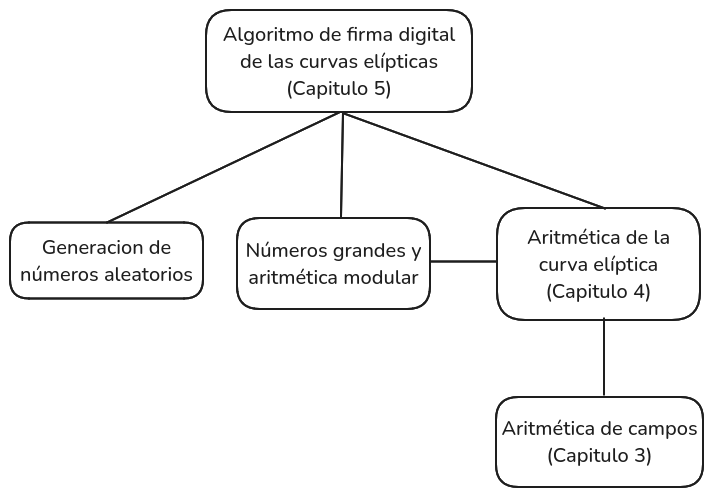
\includegraphics[width=0.8\textwidth]{imagenes/ECDSA_esquema.png}
    \caption{Esquema del Algoritmo de firma digital de las curvas elípticas (ECDSA)}
    \label{fig:ECDSA_esquema}
\end{figure}
%need to update this
La sección~\ref{sec:historia_curvas_elipticas} ofrece una introducción a las curvas elípticas donde se presentan las operaciones de grupo de suma y duplicado para los puntos de la curva, junto con su estructura fundamental y otras propiedades básicas. La sección~3.2 expone las representaciones en coordenadas proyectivas (y los algoritmos asociados de suma y duplicado), de especial interés cuando la inversión en el campo es más cara que la multiplicación. La sección~3.3 discute estrategias para la multiplicación de puntos.

Los métodos de las secciones~3.4, 3.5 y 3.6 están relacionados en que todos ellos explotan endomorfismos de la curva para reducir el coste del duplicado en la multiplicación de puntos. La sección~3.4 trata las curvas de Koblitz especiales, que permiten sustituir el duplicado de punto sobre \(\mathbb{F}_2\) por operaciones de cuadrado en el campo, mucho más baratas. La sección~3.5 examina una clase más amplia de curvas elípticas que admiten endomorfismos usados eficientemente para disminuir el número de duplicaciones. Las estrategias de la sección~3.6, para curvas sobre campos binarios, reemplazan la mayoría de los duplicados por una operación de “halving” de punto, potencialmente más rápida. La sección~3.7 recoge comparaciones de conteo de operaciones para métodos seleccionados de multiplicación de puntos. Finalmente, la sección~3.8 concluye con notas del capítulo y referencias.


\subsection{Historia}\label{sec:historia_curvas_elipticas}
Las curvas elípticas nacen del problema de calcular la longitud de arco de una elipse, que John Wallis abordó en 1655, y se articulan primero como integrales elípticas gracias a los pioneros Giulio Fagnano y Leonhard Euler en la primera mitad del siglo XVIII. En 1786, Adrien-Marie Legendre sistematiza estas integrales en tres “tipos” y sienta las bases de las funciones elípticas. A finales de la década de 1820, Niels Abel y Carl Jacobi invierten estas integrales, dando lugar a la teoría clásica de funciones elípticas. A mediados del siglo XIX, Karl Weierstrass y Bernhard Riemann las conectan con la estructura algebraico‐geométrica de curvas de género uno (tóricas complejas). Finalmente, en el siglo XX, Louis Mordell y André Weil desarrollan la teoría aritmética de puntos racionales, abriendo paso a la geometría algebraica moderna.

\section{Definición de una curva elíptica}\label{sec:definicion_curvas_elipticas}
\begin{definicion}[Curva elíptica sobre un cuerpo]\label{def:definicion_curvas_elipticas}
Sea $K$ un cuerpo. Una \emph{curva elíptica} $E$ sobre $K$ es un modelo de Weierstrass generalizado de la forma
\begin{equation}\label{eq:weierstrass_generalizada}
  E:\quad y^2 + a_1\,x\,y \;+\; a_3\,y \;=\; x^3 + a_2\,x^2 + a_4\,x + a_6,
\end{equation}
donde
\[
a_1,\;a_2,\;a_3,\;a_4,\;a_6 \;\in\; K,
\]
sujeto a la condición de no singularidad que expresaremos a continuación.

\medskip

\noindent\textbf{Invariantes auxiliares.} Definimos los siguientes invariantes:
\[
\begin{aligned}
  d_2 &= a_1^2 + 4a_2, &\quad
  d_4 &= 2a_4 + a_1 a_3,\\
  d_6 &= a_3^2 + 4a_6, &\quad
  d_8 &= a_1^2 a_6 + 4a_2 a_6 - a_1 a_3 a_4 + a_2 a_3^2 - a_4^2.
\end{aligned}
\]

\medskip

\noindent\textbf{Discriminante.} El discriminante de la ecuación \eqref{eq:weierstrass_generalizada} se define por
\[
  \Delta \;=\;-\,d_2^2\,d_8 \;-\; 8\,d_4^3 \;-\; 27\,d_6^2 \;+\; 9\,d_2\,d_4\,d_6.
\]
Con la condición necesaria $\Delta \;\neq\; 0$.

\medskip

\noindent\textbf{Punto en el infinito y conjunto de puntos racionales.}  
Denotamos por $\infty$ el único punto en el infinito (punto de Weierstrass) que completa la curva para obtener un cuerpo de funciones de género 1. Para cualquier extensión de cuerpos $L/K$, el conjunto de puntos de $E$ con coordenadas en $L$ viene dado por
\[
  E(L) \;=\; \bigl\{(x,y)\in L^2 : y^2 + a_1\,x\,y + a_3\,y - x^3 - a_2\,x^2 - a_4\,x - a_6 = 0 \bigr\}
  \;\cup\;\{\infty\}.
\]
\end{definicion}


\subsection{Comentarios sobre la definición~\ref{def:definicion_curvas_elipticas}}
\begin{enumerate}
  \item La ecuación \eqref{eq:weierstrass_generalizada} se conoce como la \emph{ecuación de Weierstrass}.
  \item Decimos que \(E\) está \emph{definida sobre} \(K\) porque los coeficientes \(a_i\) pertenecen a \(K\). A menudo escribimos \(E/K\) y diremos que \(K\) es un \emph{cuerpo base}.
  \item La condición \(\Delta\neq0\) garantiza que la curva es \emph{suave}, es decir, no tiene singularidades (no hay puntos con dos tangentes distintas). Esto esencialmente viene dado por puntos que anulan las derivadas paricales de la siguiente función de una curva elíptica:
  \[
    f(x,y) = y^2 +a_1xy + a_3y -x^3 - a_2x^2 - a_4x - a_6
  \]
  Se puede encontrar un ejemplo donde \(\Delta\neq0\) en la figura ~\ref{fig:elliptic_curve_singular_example}.
  \item El punto \(\infty\) es el único punto de la "línea en el infinito" que satisface la forma proyectiva de la ecuación de Weierstrass.
  \item Los \emph{puntos \(L\)-racionales} de \(E\) son aquellos cuyos pares \((x,y)\) pertenecen al cuerpo \(L\). Siempre incluimos \(\infty\).
\end{enumerate}

\begin{figure}[H]
    \centering
    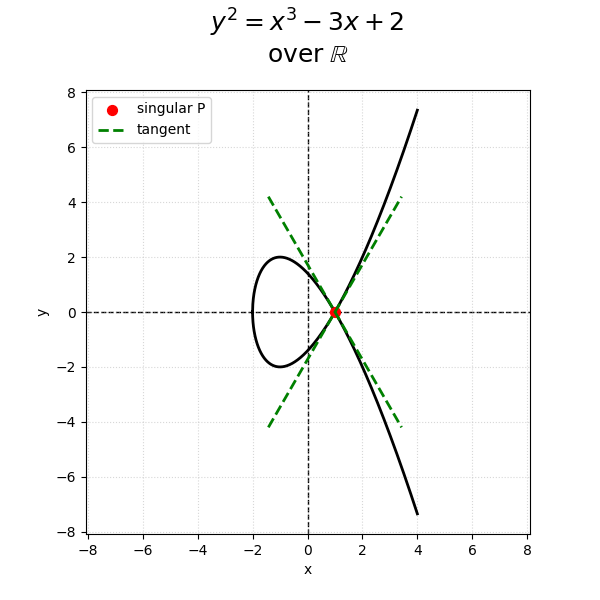
\includegraphics[width=0.8\textwidth]{imagenes/elliptic_curve_singular_example.png}
    \caption{Ejemplo de una curva elíptica con un punto singular, es decir, \(\Delta\neq0\)}
    \label{fig:elliptic_curve_singular_example}
\end{figure}

\begin{ejemplo}
Consideremos dos curvas elípticas sobre \(\mathbb{R}\):
\[
  E_1: \;y^2 = x^3 - 12x - 5,
  \qquad
  E_2: \;y^2 = x^3 + 3x + 15.
\]
Las gráficas de los conjuntos \(E_1(\mathbb{R})\setminus\{\infty\}\) y
\(E_2(\mathbb{R})\setminus\{\infty\}\) se muestran en la figura~\ref{fig:curvas_reales}.
\end{ejemplo}

\begin{figure}[H]
  \centering
  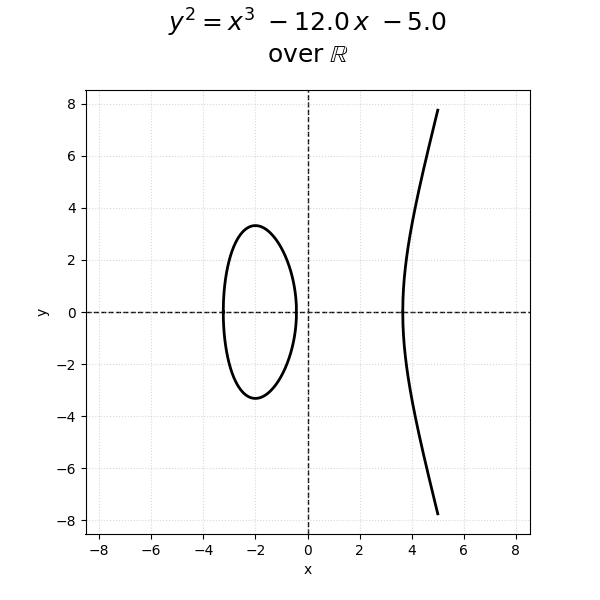
\includegraphics[width=0.48\textwidth]{imagenes/elliptic_curve2D_example.png}
  \hfill
  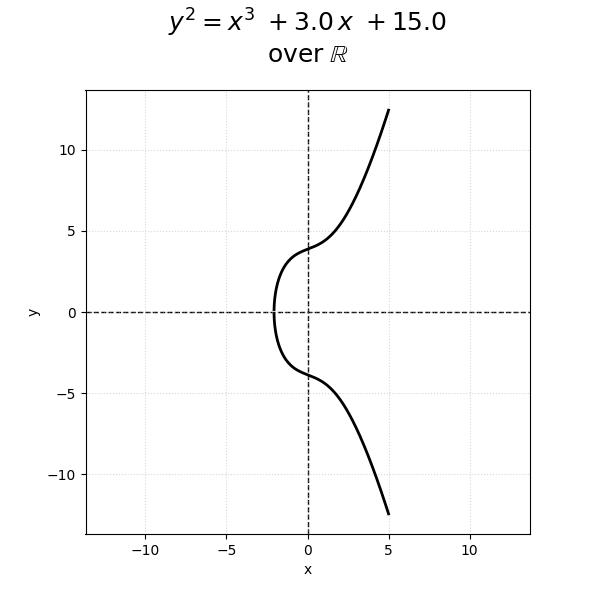
\includegraphics[width=0.48\textwidth]{imagenes/elliptic_curve2D_example2.png}
  \caption{Curvas \(E_1\) y \(E_2\) sobre \(\mathbb{R}\), con sus respectivos puntos (excepto \(\infty\)).}
  \label{fig:curvas_reales}
\end{figure}

\subsection{Forma de Weierstrass general}\label{sec:weierstrass_curvas_elipticas}
\subsection{Transformaciones y cambios de coordenadas}

\section{Estructura de grupo}
\subsection{Punto en el infinito}
\subsection{Ley de suma de puntos (geometría proyectiva)}
\subsection{Propiedades algebraicas}

\section{Curvas sobre cuerpos finitos}\label{sec:curvas_sobre_cuerpos_finitos}
\subsection{Curvas sobre \texorpdfstring{$\mathbb{F}_p$}{Fp}}\label{sec:curvas_sobre_cuerpos_finitos_primos}
\subsection{Curvas binarias sobre \texorpdfstring{$\mathbb{F}_{2^m}$}{F2m}}\label{sec:curvas_sobre_cuerpos_finitos_binarios}

\section{Coordenadas y representación}\label{sec:coordenadas_curvas_elipticas}
\subsection{Coordenadas afines}
\subsection{Coordenadas proyectivas y Jacobianas}
\subsection{Coordenadas 'mixed' y optimizaciones}

\section{Selección de parámetros}
\subsection{Tamaños de curva y seguridad}
\subsection{Cofactores y subgrupos}
\subsection{Curvas estandarizadas (secp256k1, Curve25519, …)}